\section{Evaluation}
\label{sec:eval}

Although \quicksand~presents Iterative Deepening and data-race PPs as interconnected techniques, they each could be employed alone as well. %in other model checkers.
For example, a single-state-space tool could use data-race PPs during immediately subsequent interleavings,
%essentially
changing the state space on the fly.
Likewise, a message-passing-only tool could use Iterative Deepening despite a concurrency model lacking data races, % being absent from its concurrency model.
to promote completing subset PP sets for large tests.
Hence,
we also evaluated each technique individually,
though many of our experiments compare \quicksand~to the state-of-the-art as a whole.
Our evaluation answers the following questions:
\begin{enumerate}

	\item Does \quicksand~improve upon state-of-the-art MC?
		\begin{enumerate}
			\revision{\item} Do data-race PPs expose new bugs that couldn't be found with SSS-MC's fixed-PP-set approach?
				% Elaborate later:
				% Among those, how many were missed in a {\em completed} execution of the otherwise ``maximal'' state space?
			\revision{\item} Does \quicksand~find bugs faster
				%than SSS-MC
				in subset state spaces, even without data-race PPs?
			% Probably not... ICB is state of the art here.
			% In large tests, can Iterative Deepening provide partial verification by completing smaller state spaces
			\revision{
			\item Does \quicksand~provide more full verifications of bug-free programs more quickly?
			}
			\revisionx{
			\item How does the choice between HB and Limited HB affect bug-finding and verification performance?
			}
		\end{enumerate}
	\item Does MC improve the accuracy of data-race detection?
		\begin{enumerate}
		\item Does \quicksand~avoid false positives compared to a single-execution \revisionx{Limited HB} data race analysis?
				% Explain later as:
				% How many data-race candidates were verified as benign
				% But to be fair, you have to count how many DRs are reported as "couldn't test these, check yourself" at the end.
				% Also Include:
				% How many false positives does the free-re-malloc technique suppress?
				% to do (done) If you have time, re-run all of the dr-only bug tests, with DR_FALSE_NEG enabled, and see how much fewer bugs get found (how many bugs get pushed past the time limit?)
				% Answer: Just 1. (for p2s at least; as of time of writing, pintos dr-falsenegs not run yet)
			\item Does \quicksand~find data-race bugs that would be false-negatives during a single-execution analysis?%Do we avoid false negatives compared to single-pass?
		\end{enumerate}
\end{enumerate}

%%%%%%%%%%%%%%%%%%%%%%%%%%%%%%%%%%%%%%%%%%%%%%%%%%%%%%%%%%%%%%%%%%%%%%%%%%%%%%%%

\subsection{Test Suite}
\label{sec:testsuite}
Our test suite consists of \numthrlibs~``P2'' student thread libraries, from Carnegie Mellon's 15-410 operating systems class,
and \numpintoses~``Pintos'' student kernels, from Berkeley's CS162 and University of Chicago's
\revision{CMSC 23000}~operating systems classes.
%
The P2 project comprises \texttt{thr\_create()}, \texttt{thr\_exit()}, \texttt{thr\_join()}, mutexes, condition variables, semaphores, and reader/writer locks;
all implemented from scratch in userspace with a UNIX-like system call interface \cite{kspec,thrlib}.
%
The Pintos kernel project
comprises priority scheduling, \texttt{sleep()}, and user-space process management (\texttt{wait()} and \texttt{exit()})
using provided mutex, context-switch, and virtual memory implementations
\cite{pintos}.
% P2 SLOC stats: 1807 avg; 1723 median; range 1181-4114.
% All numbers, obtained with:
% cd p2s; for i in */*; do wc -l $i/user/libthread/*.{c,h,S} $i/user/libthread/*/*.{c,h,S} ; done | grep total
% 1181 1192 1221 1230 1238 1240 1243 1261 1275 1307 1310 1318 1325 1334 1336 1345 1366
% 1388 1388 1403 1415 1416 1430 1451 1478 1498 1527 1589 1618 1635 1638 1654 1675 1676
% 1716 1719 1720 1723 1723 1727 1737 1743 1744 1751 1769 1777 1782 1789 1789 1812 1918
% 1926 1946 1994 2022 2043 2066 2077 2088 2099 2131 2164 2172 2190 2215 2227 2277 2282
% 2384 2387 2483 2486 2503 2514 2551 2597 2610 2665 4114
%Though not ``real world'' programs,
Both projects are quite complex:
the P2s average 1807 lines of code, %C and x86 assembly (stddev 489.5),
% Pintos SLOC stats: 718.1923077 avg; 643 median; range 68-1821
% Obtained with:
%function getloc {
%	diff -ru /tmp/shit/pintoses/di/src/$2/ $1/src/$2 | diffstat | grep insertions | sed 's/.*changed, //' | sed 's/ insertion.*//'
%}
%for i in `ls -d /tmp/shit/pintoses/* | grep -v -- "-p1$"`; do
%#for i in /tmp/shit/pintoses/daniel-deniz*; do
%	echo -ne "$i";
%	tloc=`getloc $i threads`
%	uloc=`getloc $i userprog`
%	dloc=`getloc $i devices`
%	echo -e "\t$tloc\t$uloc\t$dloc"
%done
and the Pintoses average 718 lines, for a total of 198,772 lines tested for this paper.

We chose P2s and Pintoses for our test suite because of the relative ease of generating hundreds of unique state spaces,
varied in size and correctness, and with a diverse set of bug types\footnote{
Many of the codebases exhibited {\em deterministic} bugs (i.e., encountered on the first interleaving tested).
We fixed these by hand, before running tests, to ensure that every bug in our study required meaningful work by the MC.}.
% TODO: Is this ok? Too arrogant?
We believe that merely finding a small handful of new real-world bugs is largely anecdotal,
and that our test suite's size allows for a more statistically significant comparison among MC and data-race testing strategies.
%compared to anecdotally showing a small handful of new bugs that could be found in real-world programs.

\newcommand\mxtest{\texttt{mx\_test}}
\newcommand\tej{\texttt{join\_test}}
\newcommand\bct{\texttt{bcast\_test}}
\newcommand\paraguay{\texttt{signal\_test}}
\newcommand\paradise{\texttt{sem\_test}}
\newcommand\rwldgr{\texttt{rwlock\_test}}
\newcommand\prisema{\texttt{sched\_test}}
\newcommand\waitsimple{\texttt{wait\_test}}
\newcommand\alarmsimul{\texttt{alarm\_test}}

We tested P2s with 6 multithreaded programs:
% from the 410 test suite % XXX: I would like to say this but this is a lie; figure out what else i can say instead
% each tailored to exercise a different part of the P2 project
\mxtest, for locking algorithm correctness,
\tej, a test of thread lifecycle,
\bct~and \paraguay~for condition variables,
\paradise~for semaphores,
% XXX f u latex
and \rwldgr\\for r/w locks.
For \mxtest, \paradise, and \paraguay, we used the {\tt without\_function} command to blacklist {\tt thr\_create}, {\tt thr\_exit}, and {\tt thr\_join},
and for \mxtest~we enabled \landslide's mutex-testing option
(see \sect{\ref{sec:landslide}}).
We tested Pintoses with 3 programs from the class's provided test suite: \prisema, a test of the kernel scheduling algorithm,
\alarmsimul, for the timer sleep routine,
and \waitsimple, for process lifecycle system calls\footnote{
	Some of the Pintoses were partially implemented,
	so each test could only be run on a subset of the 78 submissions; see ``Number tested'' in Table~\ref{tab:drbugs}.
}.
The source code of all 9 test cases is available at
{\em [submitted as supplementary material]}.
For all tests, we used {\tt without\_function} to blacklist PPs on {\tt malloc}'s internal lock.
In total, our evaluation comprises 629 unique tests (i.e., pairs of a test program and a Pintos or P2),
% at least 157 of which could expose bugs.
at least 173 of which will expose bugs under one or more MC trials. % QS bugs + bugs where SSSMC found but QS didnt

%\begin{table}[t]
%	\begin{tabular}{l|l|l}
%			& QS bugs & SSS-MC bugs \\
%		\hline
%		\mxtest & eg 1000 & eg 0 \\
%		\bct & & \\
%		etc... & & \\
%		\hline
%		Total & & \\
%	\end{tabular}
%	\caption{Comparison of all bugs found, broken down by test case, among all P2s (top 6) and Pintoses (bottom 2)}
%	\label{tab:allbugs}
%\end{table}
%
%\begin{table}[t]
%	\small
%	\begin{tabular}{l|l|l||l|l}
%	& QS bug & \begin{tabular}{c} SSS-MC \\ completed\end{tabular}
%	& QS bug & \begin{tabular}{c}SSS-MC \\ timeout \end{tabular} \\
%		\hline
%		\mxtest & e.g. 5 & 10 & 0 & 0 \\
%		\bct & & & & \\
%		etc... & & & & \\
%		\hline
%		Total & & & & \\
%	\end{tabular}
%	\caption{Bugs requiring data-race PPs to expose, found by \quicksand~but missed by the single-state-space approach.}
%	\label{tab:drbugs}
%\end{table}

%%%%%%%%%%%%%%%%%%%%%%%%%%%%%%%%%%%%%%%%%%%%%%%%%%%%%%%%%%%%%%%%%%%%%%%%%%%%%%%%

\revision{
\subsection{Experimental Setup}
\label{sec:eval-setup}

To evaluate the benefits of data-race PPs and Iterative Deepening separately, we ran the test suite under \quicksand~in \revisionx{three} different configurations, each of which was given a 1-hour budget and 10 CPUs for each test.
\begin{itemize}
		\revisionx{
	\item {\bf QS-Limited-HB}: \quicksand~using Limited HB for its data-race analysis,
	\item {\bf QS-Pure-HB}: \quicksand~using pure HB instead, and
		}
	\item {\bf QS-Sync-Only}: \quicksand~with PPs still seeded as described in \sect{\ref{sec:initial-pp}}, but never adding new PPs from reported data-race candidates.
\end{itemize}

We represented the MC state-of-the-art with 3
%different
configurations of stand-alone \landslide~on the same test suite:
\begin{itemize}
	\item {\bf SSS-MC-DPOR}: Single state space using the maximal PP set from \sect{\ref{sec:initial-pp}}, explored with DPOR \cite{dpor},
	\item {\bf SSS-MC-ICB}: With PPs as above, but instead using ICB \cite{chess-icb} with BPOR \cite{bpor} to find bugs faster, and
	\item {\bf SSS-MC-Shared-Mem}: % TODO: better name?
		Using ICB+BPOR, configured to preempt on any shared memory access \cite{inspect}
		(decided at runtime, excluding threads' accesses to their own stacks),
		which in principle includes all possible data-race PPs.
\end{itemize}
Because parallelizing DPOR/ICB during SSS-MC is an open research problem \cite{parallel-dpor},
we optimistically gave control experiments a linear speedup of 10 hours per test with 1 CPU.
%To match this,
\quicksand~reports the CPU-time spent in addition to the wall-clock time for a resource-fair comparison
(although, with the growing importance of multicore for performance, \quicksand's inherent parallelism is a convenient benefit).
%Finally,
All tests ran on 12-core 3.2 GHz Xeon W3670 machines. %with 12GB of RAM.
}

\subsection{\revision{Comparison to State-of-the-Art MC}}%Comparing Iterative Deepening to SSS-MC
\label{sec:eval-sssmc}

Figure~\ref{fig:dowefindbugsfaster} plots the cumulative distribution of bugs found \revision{by each experiment}
against the time taken to find each bug.
\revision{
Figure~\ref{fig:dowefindbugsfaster}(a) is the main, resource-fair comparison by CPU-time;
we additionally show a wall-clock comparison in (b) to highlight the impact of \quicksand's parallelism.
}

\begin{figure}[t]
	\hspace{-1em}
		\revision{
	\begin{tabular}{p{0.48\textwidth}}
	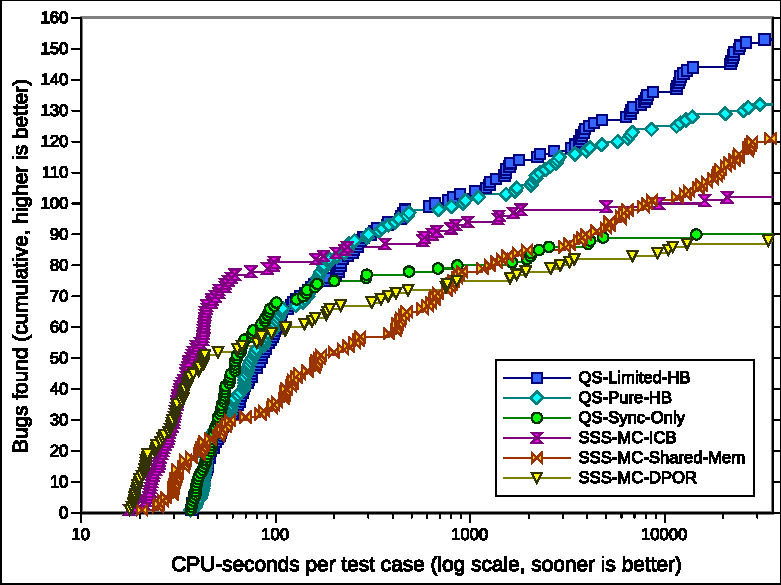
\includegraphics[width=0.48\textwidth]{dowefindbugsfaster-v2.pdf} \\
		(a) Bugs found \revisionx{as a function of} elapsed CPU time. Overall,
		a more \revisionx{resource-fair} comparison than (b),
		although \quicksand's start-up overhead is exaggerated, as the SSS-MC tests are not parallelized. \\
		\\
	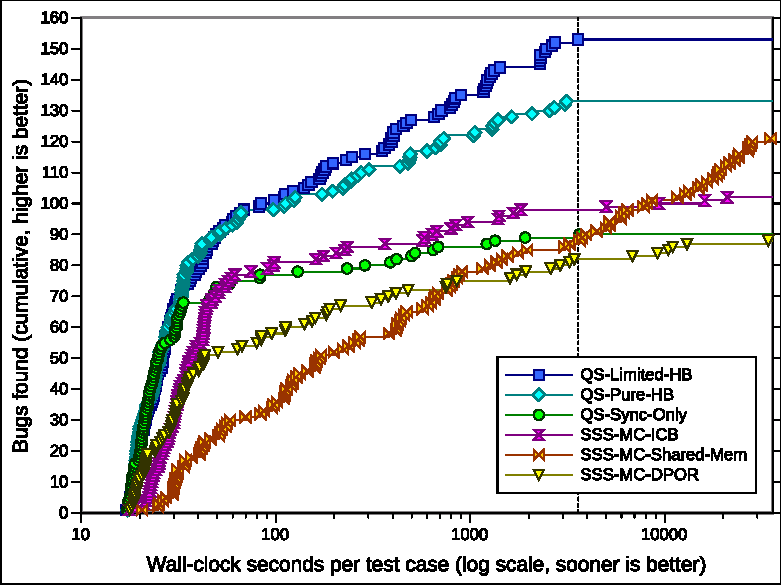
\includegraphics[width=0.48\textwidth]{dowefindbugsfaster-wallclock-v2.pdf} \\
		(b) Bugs found by elapsed wall-clock time.
		\quicksand~is parallelized tenfold; the vertical line indicates its 1 hour limit. \\
	\end{tabular}
	}
	\caption{Comparison of bug-finding performance
	by several configurations of \quicksand~and the SSS-MC control.
	\quicksand~finds \revisionx{125\%} as many bugs \revisionx{at the 10-hour mark compared to the best SSS-MC approach}.}
	%with data-race PPs.}
	\label{fig:dowefindbugsfaster}
\end{figure}

\begin{table*}[t]
	\begin{center}
		\small
		\revisionx{
	\begin{tabular}{r|c||c|c|c|c|c||c|c||c|c}
		& {\bf Num.} & {\bf QS-LHB} & {\bf QS-PHB} & {\bf ICB} & {\bf DPOR} & {\bf ShMem} & {\bf LHB DR} & {\bf Nondet.} & {\bf Mutual} & {\bf Avg. tested} \\
		{\bf Test} & {\bf tested} & {\bf bugs} & {\bf bugs} & {\bf bugs} & {\bf bugs} & {\bf bugs} & {\bf bugs} & {\bf DR bugs} & {\bf timeouts} & {\bf subset SSes} \\
		\hline
				% XXX FIXME: Need rerun nondet dr expt!
				% #test  qs-lhb  qs-phb   icb     dpor    everyw  dronly  nondets timeout comp.SSes
		{\tt bcast}	& 79	& 8	& 8	& 5	& 6	& 7	& 2	& 4	& 7	& 112.3	\\
		{\tt join} 	& 79	& 23	& 20	& 13	& 13 	& 14	& 11	& 6	& 11	& 75.9	\\
		{\tt mx} 	& 79	& 10	& 9	& 1	& 1	& 12	& 9	& 1	& 0	& -	\\
		{\tt sem} 	& 79	& 17	& 16	& 12	& 11	& 12	& 7	& 5	& 36	& 93.4	\\
		{\tt signal} 	& 79	& 10	& 8	& 5	& 5	& 11	& 6	& 6	& 45	& 59.0	\\
		{\tt rwlock} 	& 79	& 27	& 26	& 25	& 23	& 28	& 4	& 2	& 43	& 88.3	\\
		\hline
		{\tt sched} 	& 59	& 7	& 7	& 1	& 1	& 8	& 6	& 4	& 2	& 13.0	\\
		{\tt alarm} 	& 44	& 21	& 12	& 16	& 5	& 29	& 17	& 3	& 16	& 8.1	\\
		{\tt wait} 	& 52	& 30	& 27	& \revisionz{24}
								& 23	& 1	& 7	& 1	& 13	& 32.8	\\
		\hline
		{\bf Total}	& 629	& 153	& 133	& \revisionz{102}
								& 88	& 122	& 69	& 32	& 173	& 69.5 	\\
	\end{tabular}
		}
	\end{center}
	\caption{Summary of bugs
	%and data races
	found by each test program.
		\revisionx{QS-LHB and QS-PHB are \quicksand; ICB/DPOR/ShMem are the controls (\sect{\ref{sec:eval-setup}}).}
		``LHB DR bugs'' counts among \revisionx{QS-Limited-HB's} bugs how many required data-race PPs to expose (\sect{\ref{sec:eval-sssmc}});
	among those, ``Nondeterministic DR bugs'' counts how many candidates required MC integration to identify (\sect{\ref{sec:eval-dr}}).
	``Mutual timeouts'' counts how often both \revisionx{QS-Limited-HB and SSS-MC-ICB} timed out with no bug found;
	among those, ``Average tested subset SSes'' counts how many partial verifications \quicksand~provided on average for each test (\sect{\ref{sec:eval-sssmc}}).
		}
	\label{tab:drbugs}
\end{table*}

{\bf Finding new data-race bugs.}
%We quickly pull ahead of SSS-MC, and ultimately conclude with 179\% as many bugs in total.
%The break-even point is at a negligible 90 seconds.
\revision{Compared to \revisionx{SSS-MC-ICB (the fastest among the control experiments),} \quicksand~finds}~more bugs within any CPU budget greater than \revision{200}~seconds.
\revisionx{Compared to SSS-MC-Shared-Mem (the best SSS-MC approach in the long term), \quicksand's Limited HB version} ultimately concludes 10 CPU-hours with \revisionx{125\%} as many bugs in total.
\revision{Before the break-even point at 200 seconds,
\quicksand~lags behind \revisionx{SSS-MC-ICB} due to additional start-up overhead from its tenfold parallelism.
However, converting SSS-MC's early CPU-time advantage into faster wall-clock performance remains an open research problem \cite{parallel-dpor}.
Figure~\ref{fig:dowefindbugsfaster}(b) gives \quicksand~full credit for its inherent parallelism:
with a 10 core allocation, it outperforms SSS-MC
for any fixed budget of wall-clock time.}
\revisionx{After 1 hour of wall-clock time, tenfold \quicksand~performs 158\% as well as SSS-MC-ICB.}

% TODO CAMREADY
%\revision{
%%{\bf Variance.}
%% TODO CAMREADY: Probably will need at least a 3rd run of dis.
%Because \quicksand~can be nondeterministic in its scheduling of state spaces,
%we ran the QS-Limited-HB and QS-Pure-HB tests a second time to quantify the variance.
%% TODO CAMREADY
%% We found the maximum area between any two curves to be
%We found the area between the two curves to be
%% TODO CAMREADY
%{\bf XX\%}
%of the area between QS-TODO(?)-HB and SSS-MC-Shared-Mem (the next closest),
%% TODO cite CAMREADY
%which we consider an insignificant amount of variance.
%}

% TODO: Fix up this paragraph after preempt-everywhere results come in.
The left half of Table~\ref{tab:drbugs}
breaks down the number and types of bugs found by each test program.
In \mxtest, in which we do not trust the lock implementation's correctness,
% TODO CAMREADY: Fix, SSSMC-ShM finds 2 mx bugs.
\revisionx{SSS-MC-ICB and SSS-MC-DPOR}
found dramatically fewer bugs (just 1)\footnote{
	The one bug SSS-MC found was in a fully-assembler lock implementation. {\tt yield()}'s return value clobbered a value stored in {\tt \%eax}, which could lead to a failure after two repeated contentions. Preempting only on {\tt yield()} (in the contention loop) was sufficient to find the bug.}.
%Intuitively, this is due to our control experiment being able to preempt only on the boundaries of the API which
%Though for many applications of MC, assuming a correct lock implementation is sufficient,
Though it often suffices to assume correctly-implemented locks \cite{dbug-thesis},
we consider this strong evidence that new low-level synchronization code must be verified with data-race PPs.
%TODO CAMREADY: Run a mutex expt where "all atomic instrs" are PPs. See how many bugs are missed anyway.
% Wwe re-ran the \mxtest control experiment with \landslide~hard-coded to preempt on any atomic instruction
% (as well as on the mutex API boundaries).
% Still, this smarter configuration for SSS-MC found only 99999999999 bugs of \quicksand's 13.

%% RIP this.
%Furthermore, we plotted another line from this dataset, QS-no-DR-bugs,
%which represents only the bugs found in state spaces without any data-race PPs (like QS-no-DR-PPs, but paying any overhead for using data-race PPs).
%Intuitively, this line shows that for programs with only benign data races,
%\quicksand~can afford the extra overhead of verifying them while still slightly edging out SSS-MC.

% TODO CAMREADY: Compare QS-ETAs to QS-Random to evaluate "smaller is better" claim.
{\bf Finding the same bugs faster.}
%To test whether Iterative Deepening is effective even for MC domains without data races, %such as message-passing distributed systems,
\revision{The QS-Sync-Only experiment tests whether}~Iterative Deepening is effective even for MC domains without data races.
\revision{When \quicksand~ignores all data-race candidates,
its results are competitive with SSS-MC-DPOR, but SSS-MC-ICB outperforms it.
This is unsurprising: the seed subsets of PPs
QS-Sync-Only is limited to
(\sect{\ref{sec:initial-pp}})
are much less flexible than ICB's preemption strategy (\sect{\ref{sec:overview-sssmc}}).
This result suggests that in future work, \quicksand~should consider using ICB in parallel with its default configuration when it finds no data-race candidates to test.}
%\footnote{
%Because \quicksand~is not yet instrumented to subset hard-coded PPs beyond the 4 ways shown in Figure~\ref{fig:id},
%we ran these tests for 2.5 hours on 4 CPUs each.
%Future work could parallelize QS-no-DR-PPs further; see \sect{\ref{sec:future}}.}.

%Even though SSS-MC mostly catches up to it by the end of the 10-hour budget,
%and is faster in the first 60 seconds due to less start-up overhead,
%QS-no-DR-PPs finds more of the bugs sooner thereafter.
%Hence, for modest CPU budgets,
%\quicksand~is likely to find bugs SSS-MC will miss.
%and for more ambitiously-sized tests,
%programmers can be more confident in the verification provided when \quicksand~times out with no bug found.
%We conclude that for smaller arbitrary CPU budgets, especially less than 1 hour,
%Iterative Deepening is likely to find bugs SSS-MC will miss.
%Moreover, it is also easy to imagine scaling up the size of each test case to test ,
%using more threads or longer sequences of API calls.
%We hope that is compelling even to users willing to spend many CPU-hours on testing.
%These results show explicitly that for arbitrary CPU-time budgets
%\footnote{The initial perfect overlap between QS-*-HB and QS-Sync-Only indicates how long it takes before the first data-race bug is found.}
%even after the extra overhead of verifying them, \quicksand~still slightly edges out SSS-MC

\revision{
On the other hand,
comparing \revisionx{QS-Limited-HB} to SSS-MC-Shared-Mem shows that Iterative Deepening thoroughly outperforms ICB when shared-memory preemptions come into play.
%We attribute this to the fact that
Statically configuring a PP for every shared memory access in advance
produces orders of magnitude more PPs than
waiting for an access to be identified as part of a (potential) data race at runtime.
%
In principle, DPOR and BPOR should identify and prune any equivalences arising from extraneous PPs on non-conflicting accesses.
However, in practice,
%we found that
the sheer number of accesses during each new execution
(often thousands)
added significant performance overhead to the MC when computing DPOR and backtracking.
Iterative Deepening avoids this overhead by waiting until runtime to identify fewer, more relevant PPs dynamically,
and is hence more suitable for MC with data-race PPs.}

\revisionx{
To ensure that our corpus of P2 and Pintos bugs gives an unbiased comparison between \quicksand~and ICB,
we also counted the preemption bounds necessary for ICB to find each of its bugs.
Table~\ref{tab:icb-bounds} shows the distribution of these bounds,
which is consistent with the results of \cite{chess-icb}, showing no bias towards bugs that would be harder for ICB to find.
%justifies that our portrayal of ICB is fair.
%and shows no bias towards requiring high preemption bounds.
}

\begin{table}[h]
	\begin{center}
		\revisionx{
		\small
	\begin{tabular}{r|c|c}
		{\bf Bound} & {\bf SSS-MC-ICB} & {\bf SSS-MC-Shared-Mem} \\
		\hline
		0	& 2	& 1	\\
		1	& 82	& 86	\\
		2	& \revisionz{16}	& 32	\\
		3	& 2	& 3	\\
		4+	& 0	& 0	\\
		\hline
		Total	& \revisionz{102}	& 122	\\
	\end{tabular}
		}
	\end{center}
	\caption{\revisionx{Distribution of preemption bounds among bugs found by ICB control experiments. (Bound 0 means the bug was found by switching threads only on {\tt yield()}s.)}}
	\label{tab:icb-bounds}
\end{table}

{\bf Partial verification.}
When a MC job times out, the user may prefer a brief summary of what parts of the test were verified, rather than writing off all the CPU time as a waste.
%Beyond using the state space estimator to guess the percent coverage,
%We know of no approach to quantify the probability
%that a bug would be exposed by an untested interleaving,
While recent work \cite{randomized-scheduler} attempts to quantify the probability
that an untested interleaving would expose a bug,
\quicksand~instead reports which subsets of PPs resulted in state spaces that did complete in time.
%\quicksand~does not attempt any such quantitative guarantee,
%but can at least report
On \revisionx{310} tests, \revisionx{SSS-MC-ICB} timed out after 10 hours with no bugs found.
Among these tests, \quicksand~found bugs in \revisionx{47}.
For the other \revisionx{263}, we show the number of state spaces \quicksand~was able to complete in the ``Average tested subset SSes'' column of Table~\ref{tab:drbugs}.
%and the number of unique PPs among them.
%In 6 cases, \quicksand~also failed to complete anything; beyond these,
%between 1 and 253 state spaces were completed for each test
%Between 0 and 233 unique PPs were tested among some completed subsets, with a mean of 27.2 and median of 7.5.
These completions guarantee that, if the test program could expose a bug,
% Justify implicit hypothesis: Sync PPs + DR PPs = all possible relevant PPs.
it would only be found by a new data-race PP not discovered yet, or by a superset combination of PPs not reached.
\revision{
%While obviously not as strong as full verification,
Prior work \cite{sealing} has argued the value of similar {\em compositional testing} when full verification is intractable,
deferring to the user's expertise to judge the value of each subset of PPs verified.
}

%Hence, in Table~\ref{tab:drbugs} we count how often \quicksand~uncovered a bug only in state spaces which included data-race PPs, while
%
%In Table~\ref{tab:allbugs} ....

{\bf Full verification.}
For 153 of our 629 tests, \revisionx{QS-Limited-HB} was able to provide the total verification guarantee described in \sect{\ref{sec:totalverif}},
\revisionx{and QS-Pure-HB completed a verification for 167 tests.}
In Figure~\ref{fig:totalverif} we plot the cumulative distribution of
%total
verifications provided by each approach.
\revisionx{The next best approach for verifications was SSS-MC-Shared-Mem, which completed its search in only 39 cases.}

%Though SSS-MC-Shared-Mem appears to outperform \quicksand, its safety guarantee is unsound,
%as many tests break its assumption of stack-allocated memory being private.
%For example, many P2 condvars use stack-allocated list nodes to track waiting threads.
%While SSS-MC-Shared-Mem must avoid excessive PPs on every private stack access for performance,
%\quicksand~detects these dynamically, without needing to discriminate between stack and heap.
%In total, SSS-MC-Shared-Mem claimed to verify 21 tests
%(across 7 of the 9 test cases)
%in which QS-DR ultimately found bugs,
%which further calls into question the rest of its completions.

% NB. TODO CAMREADY. If a reviewer asks, "How come SSSMC-ShM completed so many state spaces,
% even though last section you argued that so many PPs slows it down terribly?"
% The answer is, "Actually, it's not that SSSMC-ShM magically got fast again for the verification experiment;
% it's that SSSMC-ShM and Quicksand are *BOTH* slow to achieve full completion.
% Quicksand can get bogged down in a combinatorial explosion of different subsets of PPs,
% having a zillion jobs on its hands. Future work should improve this with https://github.com/bblum/landslide/issues/216 ."

%\quicksand's total verifications
%%before a given elapsed CPU consumption.
%\revision{against those provided by SSS-MC-Shared-Mem\footnote{
%	\revision{In kernel or thread library code, a thread's own stack accesses may not always be private. %assumption may not hold.
%	For example, many P2 condvars use stack-allocated list nodes to track waiting threads.
%	SSS-MC-Shared-Mem's verifications are only sound in the absence of such sharing!
%	\quicksand~detects these dynamically, without needing to discriminate between stack and heap.}
%	%Expanding the statically-coded PPs to include stack accesses would make SSS-MC-Shared-Mem's performance even worse.
%	% Especially for testing kernel-level code, deciding which of a thread's memory accesses are shared versus private is nonstraightforward, as threads may share data structures allocated on their own stacks for synchronization. Hence, the common heuristic of ignoring stack accesses as private (which we employ for this control experiment) introduces some unsoundndess.
%}.
%\quicksand~outperforms SSS-MC, being able to verify safety for
%{\bf 9999x}
%as many tests in 10 CPU-hours.
%We attribute this again to the overhead of the sheer number of statically-coded PPs that SSS-MC-Shared-Mem must use,
%as well as to the work which ICB necessarily repeats when increasing its preemption bound.}

% TODO: Update for pure HB (need a re-run of a subset of completed sssmc tests to confirm they still have no pure hb drs, even if they had limited hb drs)
Among \revisionx{QS-Limited-HB's} verified tests, 36 contained no data-race candidates whatsoever,
so the same verification could be provided
%by SSS-MC
\revision{with synchronization PPs only.
We plot the verifications by QS-Sync-Only, SSS-MC-DPOR and SSS-MC-ICB as well:
among these, the otherwise more antiquated SSS-MC-DPOR performs best,
while the other two lag behind}
%\quicksand~is slower than SSS-MC-DPOR
due to redundant work (\sect{\ref{sec:future}}).
\revision{While QS-Sync-Only and SSS-MC-ICB are competitive with each other},
using data-race PPs increases our \revision{verification capacity}~by 4.25x.
\revisionx{Finally, assuming sequentially-consistent hardware,
QS-Pure-HB classified many % TODO: how many
true data races as benign, %(non-failing),
while the SSS-MC-ICB approach could at best report such races to the user.
We count these cases in Table~\ref{tab:drstatistix}.
}

% Actually, while SSS-MC-Shared-Mem proved competitive with \quicksand~at finding data-race-related bugs,
% its heuristic to ignore threads' own stack accesses introduces unsoundness.
% <Move contents of footnote here.>
% Indeed, SSS-MC-Shared-Mem claimed a full verification on 999999 tests for which \quicksand~found bugs!
% % Hence, no SSS-MC strategy competes with quicksand for truly sound verification
% Hence, only SSS-MC-DPOR and SSS-MC-ICB compete with \quicksand for sound verification, and they are thoroughly outperformed.
% Between data-race bugs and verifications, \quicksand~is shown to provide the best of both worlds.

\begin{figure}[t]
	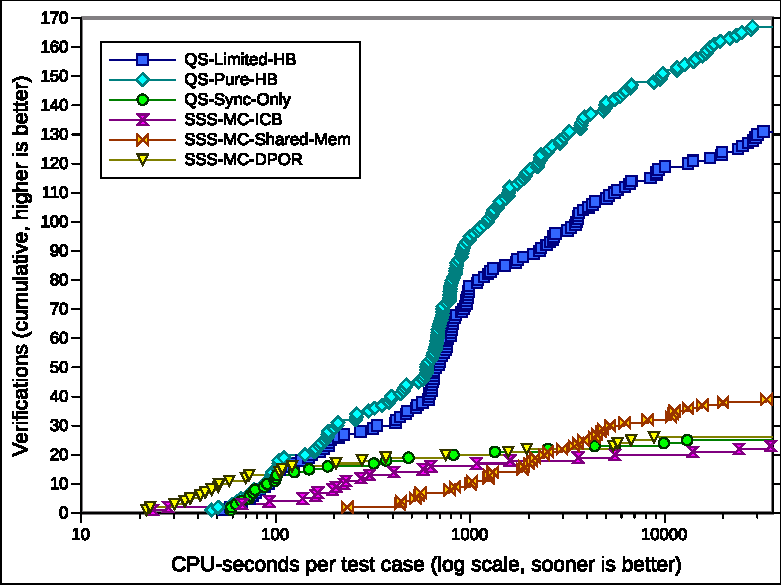
\includegraphics[width=0.48\textwidth]{totalverifs-v2.pdf}
	\caption{Cumulative distribution of tests fully verified
	\revisionx{by QS-Limited-HB, QS-Pure-HB, and SSS-MC-Shared-Mem}
	(\sect{\ref{sec:totalverif}}).
	%SSS-MC-Shared-Mem completed 1.37x as many tests, but 
	%SSS-MC-Shared-Mem is unsound: 21 tests it completed hid bugs previously found in Figure~\ref{fig:dowefindbugsfaster}.
	%previously found (Figure~\ref{fig:dowefindbugsfaster}).
	%Some tests had no data-race candidates, and hence could also be verified by .}
	36 data-race-free tests were also soundly verified by QS-Sync-Only, SSS-MC-DPOR, and SSS-MC-ICB.}
	\label{fig:totalverif}
\end{figure}

\revisionx{
{\bf Happens-Before comparison.}
Ultimately, using Limited HB for finding data-race candidates allowed \quicksand~to find more bugs, while
the ``pure'' Happens-Before analysis improved \quicksand's performance on verifications.
This trade-off is attributable to the fact that QS-Limited-HB need not wait to test many alternate thread interleavings before a potential data-race candidate is confirmed; rather, it can add new jobs to start testing potential races immediately\footnote{
	\revisionx{Table~\ref{tab:drbugs} corroborates: the difference is most dramatic in {\tt alarm}, the test where \quicksand~struggled most to finish even small subset jobs.}
	}.
On the other hand, QS-Limited-HB can get overwhelmed by too many false positives, needing to refute such candidates by testing new state spaces,
while QS-Pure-HB can refute false positives {\em en passant} by testing alternate interleavings in its original state spaces.
%In both cases, the performance differences seem to become significant only after about 10 minutes of CPU time,
%which suggests... I don't actually know!
This suggests that
%each approach has merit, and that
MCs which feature data-race analysis should implement both modes and offer the user to choose based on their testing philosophy.
}

\begin{table}[t]
	\begin{center}
		\small
		\revisionx{
	\begin{tabular}{r||c|c|c||c}
		& {\bf Total} & {\bf \revisionx{Benign}} & {\bf Untested} & {\bf Malloc} \\
		{\bf Test} & {\bf DR PPs} & {\bf \revisionx{DRs}} & {\bf DR PPs} & {\bf DRs} \\
		% note: if you wanted to calculate total DR PPs with FAB tests included, here's the nums instead:
		% alarm 66
		% bct 849
		% mx 1193
		% paradise/sem 1201
		% paraguay/signal 1088
		% sema 101
		% dgr 846
		% tej 1029
		% wait 196
		\hline
				% DRPPs   benign untested FRMs
		{\tt bcast}	& 655	& 97	& 150	& 52	\\
		{\tt join} 	& 566	& 68	& 249	& 338	\\
		{\tt mx} 	& 911	& 127	& 44	& 7	\\
		{\tt sem} 	& 783	& 2	& 414	& 166	\\
		{\tt signal} 	& 936	& 9	& 510	& 180	\\
		{\tt rwlock} 	& 543	& 1	& 310	& 156	\\
		\hline
		{\tt sched} 	& 65	& 51	& 3	& 0	\\
		{\tt alarm} 	& 35	& 0	& 29	& 35	\\
		{\tt wait} 	& 71	& 1	& 28	& 31	\\
		\hline
		{\bf Total}	& 4565	& 356	& 1737	& 965	\\
	\end{tabular}
		}
	\end{center}
	\caption{
		\revisionx{Additional data race statistics.}
		``Total DR PPs'' counts how many unique data-racing instructions \revisionx{QS-Pure-HB identified} among tests
		where it found no bugs.
		Among those,
		\revisionx{``Benign DRs'' counts how many we refuted as non-failing (\sect{\ref{sec:eval-sssmc}}), while}
		``Untested DR PPs'' counts how many could not be checked in the time limit (\sect{\ref{sec:future}}).
		``Malloc DRs'' counts how many \revisionx{false positive PPs QS-Limited-HB} suppressed (\sect{\ref{sec:eval-dr}}).
		}
	\label{tab:drstatistix}
\end{table}

%%%%%%%%%%%%%%%%%%%%%%%%%%%%%%%%%%%%%%%%%%%%%%%%%%%%%%%%%%%%%%%%%%%%%%%%%%%%%%%%

\subsection{Comparing to Single-Pass Data-Race Analysis}
\label{sec:eval-dr}
% Though we mechanically verify whether each data race candidate leads to a bug, each new PP can increase combinatorially..... obviously wish to avoid...

Beyond finding new bugs and completing full verifications with data-race PPs, we evaluated \quicksand's performance for classifying data-race candidates in two ways.

{\bf Suppressing ``malloc-recycle'' false positives.}
In \sect{\ref{sec:recycle}} we showed the soundness of suppressing data race reports between two heap accesses when the surrounding memory was re-allocated in between.
In Table~\ref{tab:drstatistix}, the column ``Malloc-recycle DRs'' shows the total number of such data-race candidates for each test program.
In total, 902 data-races fit the malloc-recycle pattern across all tests,
only 69 of which were observed to avoid the re-allocation in an alternate interleaving.
Our proof in \sect{\ref{sec:recycle}} guarantees the safety of pruning all 833 other state spaces.

Among those 69 true data-races, %which initially fit the malloc-recycle pattern,
none exposed a new bug when used as a PP.
This suggests that for other data-race tools,
suppressing malloc-recycle candidates may be a productive heuristic,
even if unsound without Iterative Deepening.
However, \quicksand~was able to correctly identify the 69 violations of that heuristic (among 30 distinct tests),
and fall back to classifying them with DPOR.
%which we consider a much stronger verification.

%%%%%%%%%%%%%%%%%%%%%%%%%%%%%%%%%%%%%%%%%%%%%%%%%%%%%%%%%%%%%%%%%%%%%%%%%%%%%%%%

%For the [NONDET] expt, you don't need to additionally count how many DRs
%needed to be found in a DR-PP state space, because when EXPLORE_BACKWARDS=0,
%you'll need to preempt on the DR PP to find the new DR anyway, hence they will
%be nondet. Unless you want to separately count the subset of nondet drs that
%are also dr-pp-ss-only (the reviewers may ask for this before cam-ready?).
{\bf \revision{Finding nondeterministic data-race candidates}.}
Some memory accesses may be hidden in a control flow path that requires a nondeterministic preemption to be executed.
In such cases, a single-pass dynamic data-race detector
%could not achieve the coverage necessary
could fail
to identify a racing access pair as a candidate at all. %to begin with.
%
We counted how many such data-races, used as PPs, led to \quicksand~finding new bugs,
thereby making them {\em false negatives} of the single-pass approach.
We classified each data-race candidate according to whether \landslide~reported them during the first interleaving,
before any backtracking or preempting:
if so, they were {\em single-pass data races}; otherwise, {\em nondeterministic}.

To ensure a fair comparison, we disabled \landslide's {\em false-positive}-avoidance techniques during this experiment.
For example, we reported malloc-recycle data races during the first interleaving, as a single-pass analysis must
%rather than waiting until future interleavings to witness them without the malloc-recycle pattern
(\sect{\ref{sec:recycle}}).
This prevents \landslide~from suppressing an observed data race on the first interleaving,
which would falsely classify it as nondeterministic.

\begin{figure}[t]
	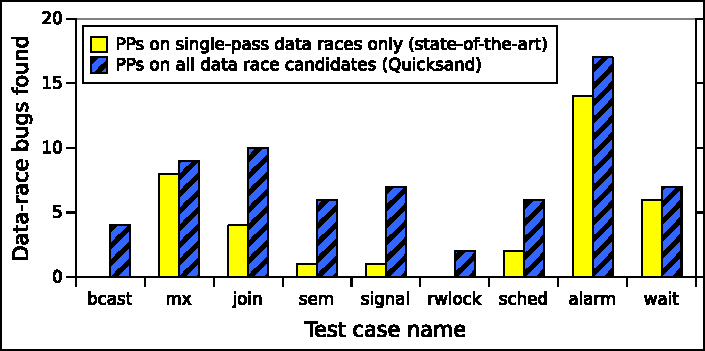
\includegraphics[width=0.48\textwidth]{nondet-drs-1-v2.pdf}
	\caption{Some data-race candidates may not be identified during a single program execution.
		Using nondeterministic data races as PPs,
		\quicksand~found 189\% as many data-race bugs compared to using single-pass candidates alone.
	}
	\label{fig:dr-falsenegs}
\end{figure}
Figure~\ref{fig:dr-falsenegs} compares the types of data-race candidates necessary to expose each data-race bug in our test suite.
The first series represents the bugs found using PPs from single-pass data-race candidates,
% not entirely true, as portend could be given data-race traces from an MC,
%but they don't do it in their paper, so i feel comfortable making this claim
i.e., the state-of-the-art approach used by \cite{racefuzzer,portend}.
The second series shows all data-race bugs \quicksand~found,
which includes the former type as well as new bugs involving nondeterministic data-races.
\quicksand~found 68 data-race bugs in total, only 36 of which could be found with single-pass data-race candidates alone.
%In total, we found 189\% as many bugs by using nondeterministic data-race candidates as PPs.

%When proving that [NONDET] dr buges exist, make sure to mention that, although
%their frequency varies depending on test case (mx test: almost none; bct:
%almost all), they are still PRESENT in all (or almost all) test cases, meaning
%it is not just a matter of writing better test cases.

Note that we are not comparing how much testing time is required before identifying the data-race candidates involved in each bug.
Single-pass data races can all be found after a single program execution,
while \quicksand~may potentially take up to all 10 CPU-hours before identifying a nondeterministic data race.
However, prior work data-race tools \cite{tsan}, being not integrated with a MC,
are not intended to discover new candidates under subsequent runs.
Running a single-pass data-race tool repeatedly for 10 CPU-hours could potentially uncover some nondeterministic candidates,
but stress testing's comparative problem with achieving reliable coverage is already well-understood
\cite{chess-icb,gambit}.
Likewise, replay-based tools \cite{portend} are dependent upon the data-race detector to provide an execution trace leading to each candidate.
This result suggests that
such tools could benefit from a similar feedback loop as is used in Iterative Deepening.
%i.e., discovering transitively-reachable data races while testing initial ones.
%although that would still not simultaneously be able to provide total verifications.
% TODO: read gambit paper


% Figure out concretely what the data race tricks are that we do, so we can claim them as contributions in the paper. Then ACTUALLY EVALUATE THEM.
%         - Speculative DR PPs.
%                 Not a heuristic, rather how to make it work at all to begin with.
%                 (Cite MS thesis, claim on backwards explorating finding bugs faster)
%         - Free/re-malloc to eliminate some false positives. See #193.
%                 Measure how many false positives are eliminated.
%                 Check, ofc, to make ABSOLUTE SURE, that no bugs missed w/ this trick.
%                         If there are, it could be because of the implementation
%                         bug described in #193.
%         - Using tid/last_call filtering because whole stack traces are too expensive.
%                 Moderately optional, 1st priority since theoretically interesting:
%                 Turn on/off and measure how resulting DR bug #s change.
%         - Optional: Reprioritizing DRs based on "confirmed" / "suspected"
%                 Shouldn't be hard just make ID wrapper print "s" or "c"!
%                 Is it helpful for ID to put priorities on DR PPs?
%                         Test by inverting the priority and see if fewer buges are found.
%         // Super optional to talk about. Probably not worth the time.
%         // - "Too suspicious" (during init/destroy)
%         //      (Cite eraser, section 2.2)
